\documentclass[10pt,twocolumn,letterpaper]{article}

\usepackage{cvpr}
\usepackage{times}
\usepackage{epsfig}
\usepackage{graphicx}
\usepackage{amsmath}
\usepackage{amssymb}
\usepackage{caption}
\usepackage{subcaption}
\usepackage{booktabs}
\usepackage{makecell}
\usepackage{algorithm}
\usepackage[noend]{algpseudocode}

% Include other packages here, before hyperref.

% If you comment hyperref and then uncomment it, you should delete
% egpaper.aux before re-running latex.  (Or just hit 'q' on the first latex
% run, let it finish, and you should be clear).
\usepackage[pagebackref=true,breaklinks=true,letterpaper=true,colorlinks,bookmarks=false]{hyperref}

%%%%%%%%% PAPER ID  - PLEASE UPDATE
\def\cvprPaperID{0947} % *** Enter the CVPR Paper ID here
\def\httilde{\mbox{\tt\raisebox{-.5ex}{\symbol{126}}}}

\begin{document}

%%%%%%%%% TITLE - PLEASE UPDATE
\title{Rebuttal for `Guided Proofreading of Automatic Segmentations for Connectomics'}  % **** Enter the paper title here

\maketitle
\thispagestyle{empty}

Thank you for your time and constructive comments. We will fix all minor issues.

\paragraph{R2: Quantitative Evaluation}
R2 requests an objective quantitative evaluation. Fortunately, our `automatic' and `oracle' experiments are exactly this. We define such experiments in lines 573--590 and report the results in Fig.~6, Fig.~7, and lines 792--818 (also in supplemental Sec.~2 and 3). These evaluations use the quantitative VI metric against a ground truth segmentation, with no user in the loop.

\paragraph{R2: Faster than State of the Art?}
%We report the average correction times for novice users in lines 756-765. Figure 7 (column 3) shows VI reduction after 30 minutes and the slopes in figure 6 also indicate better performance for GP. However, this presentation is not ideal and 
`Faster' here considers both how long each correction takes, and the likely VI reduction from that correction. Our approach has comparable correction time to the state-of-the-art Focused Proofreading appraoch, but a significantly greater VI reduction per correction (7.5$\times$). Our presentation of this discovery could have been improved. We will add Table~\ref{tab:correctiontimes} to make this clearer (previously reported in lines 756-765, slopes in Fig.~6, and column 3 in Fig.~7).

\begin{table}[h]
\caption{Average proofreading speed for users of Dojo, Focused Proofreading (FP) and our Guided Proofreading (GP). For comparable correction time, our system achieves significantly higher VI reduction per minute (7.5$\times$) over state-of-the-art FP.}%While the training of our classifier is more expensive, testing accuracy is superior. }
\resizebox{\linewidth}{!}{
\begin{tabular}{lrrrr}
\toprule
Approach & \makecell{Time Per Correction (s)} & \makecell{VI Reduction Per Minute} \\
\midrule
\emph{Dojo} & 30.5 & -0.002 \\
%\emph{Dojo Expert?} & xxx & xxx \\
\emph{FP} & 4.9 & 0.00023 \\
\emph{GP} & 6.2 & 0.00173 \\
\bottomrule
\end{tabular} 
}
\label{tab:correctiontimes}
\end{table}

\paragraph{R2: Reproducibility}
R2 expresses concerns regarding reproducibility. As per line 847, we have promised to release all our code and data, and we disclose all parameters.

\paragraph{R2: How were Optimal Parameters chosen?}
The \textbf{threshold $p_t=0.95$} was observed to be stable when evaluating on previously-unseen test data (lines 585-586, supplemental Sec. 1.3). The \textbf{input border is dilated by 5 pixels} to consider slight edge ambiguities and to cover extra-cellular space between segments in high-resolution electron microscopy data (lines 308-310). During merge error detection, \textbf{labels are dilated by 20 pixels} prior to finding potential borders (line 323) with border-seeded watershed---this way the borders tend to attach to real membrane boundaries (lines 364-366). As we use a CNN, there are many additional parameters; we consider choosing these effectively to be an open problem, and for this we used learned experience and local brute-force searches.
%Here, we list all parameters and describe how their values are obtained. We will synchronize this information with the paper.
%We define several parameters in the paper. However, we agree with reviewer 2 that finding the optimal values requires better explanations and we will synchronize the following information with the paper. 

%
%\begin{itemize}
%\item \textbf{Threshold $p_t$.} The threshold $p_t=0.95$ was observed to be stable when evaluating on previously unseen testing data (lines 585-586, supplemental Sec. 1.3).
%\item \textbf{Dilated Boundary Input.} We dilate the border between segments by 5 pixels to consider slight edge ambiguities and to cover extra-cellular space between segments in high-resolution electron microscopy data (lines 308-310).
%\item \textbf{Dilated Label.} During merge error detection, labels are dilated by 20 pixels prior to finding potential borders (line 323) with border-seeded watershed. By doing so, the borders tend to attach to real membrane boundaries (lines 364-366).
%\end{itemize}

%\begin{table}[h]
%\caption{Parameters of GP, their values and how these values are obtained.}%While the training of our classifier is more expensive, testing accuracy is superior. }
%\resizebox{\linewidth}{!}{
%\begin{tabular}{l}
%\toprule
%Threshold $p_t=0.95$, Observed on previously unseed testing data (lines 585-586, supplemental Sec. 1.3) \\ 
%\bottomrule
%\end{tabular} 
%}
%\label{tab:parameters}
%\end{table}

\paragraph{R3: Training Datasets---U-net vs.~GP?}
R3 raises the question of whether our GP approach was trained on the same data as membrane detection (U-net). There was no overlap (Tab.~\ref{tab:trainingdata}).

\begin{table}[h]
\caption{Training data of membrane detection vs.~training data of GP (for supplemental material).}%While the training of our classifier is more expensive, testing accuracy is superior. }
\resizebox{\linewidth}{!}{
\begin{tabular}{lrrrr}
\toprule
%Dataset & \makecell{Training Set\\Membrane Detection (U-Net)} & \makecell{Training Set\\Guided Proofreading} \\ 
Dataset & \makecell{Training Set\\U-Net} & \makecell{Training Set\\GP} \\ 
\midrule
\makecell{\emph{L. Cylinder}\\~} & \makecell{AC3+AC4\\($1024\times1024\times175$vx)} & \makecell{L. Cylinder\\($2048\times2048\times250$vx)} \\ 
\makecell{\emph{AC4 subvolume}\\~} & \makecell{AC4 excl. test\\ ($1000\times1000\times90$vx)} &  \makecell{L. Cylinder\\ ($2048\times2048\times250$vx)} \\ 
\makecell{\emph{CREMI A/B/C}\\~} & \makecell{AC3+AC4\\($1024\times1024\times175$vx)} & \makecell{CREMI A/B/C\\($1250\times1250\times300$vx)} \\ 
\bottomrule
\end{tabular} 
}
\label{tab:trainingdata}
\end{table}




\paragraph{R3: Merge Error Detection}
R3 requests a better explanation of the merge error detection (Sec. 3.2). We have updated Figure 4 in the main paper to be more descriptive (Fig. 1). We will also add pseudo code of the algorithm to the supplemental material to promote understanding (Alg. \ref{code:mergeerror}).

\begin{figure}[h]
\centering
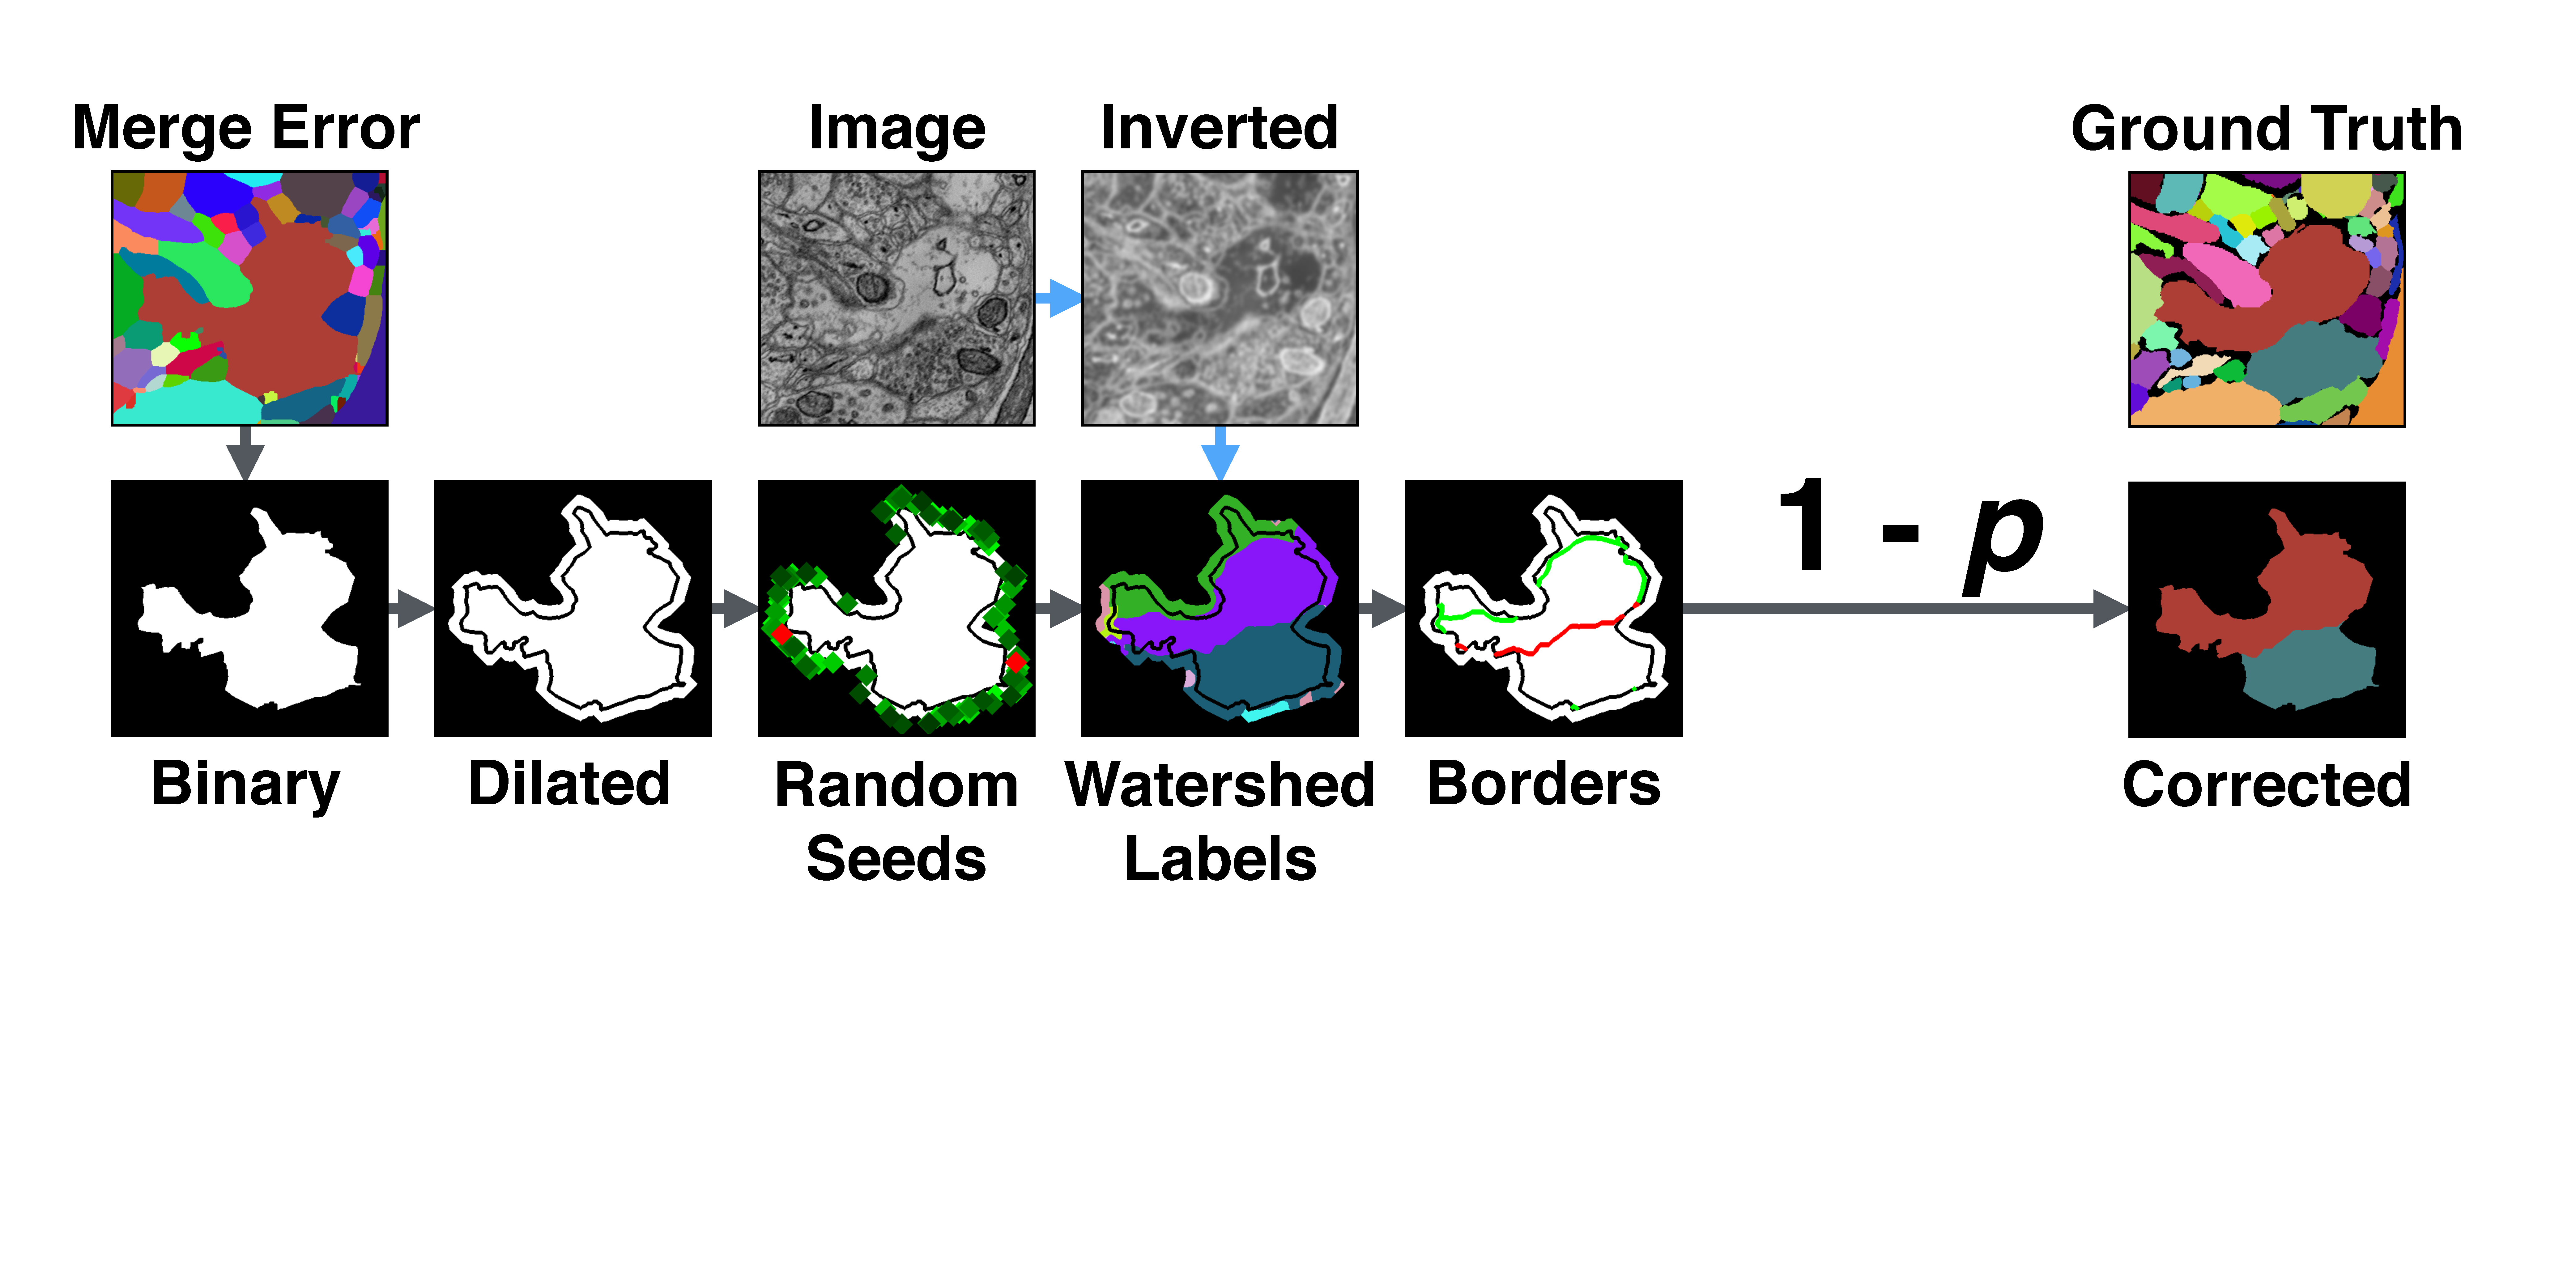
\includegraphics[width=\linewidth]{gfx/merge_error_v6.pdf}
\caption{Merge errors are identified by generating randomly-seeded watershed borders within a dilated label segment. Then, each border is individually rated using the split error CNN by inverting the probability score.}
\label{fig:merge_error}
\end{figure}

%\begin{algorithm}
%\caption{Merge Error Detection for label \emph{l}}\label{code:mergeerror}
%\begin{algorithmic}[1]
%%\State{mergeErrors = []}
%%\For{\emph{l} in $\forall$labels}
%	\State{$l_d$ = dilate(\emph{l}, 20)}
%	%\For{N iterations}
%		%\State{$s_1$,$s_2$ = findRandomSeeds($l_d$)}
%		\State{border = watershed($l_d$, $\text{seeds}_\text{random}$)}
%		%\State{border = findBorder(ws)}
%		\State{$p_\text{split}$ = rank(border)}
%		\State{$p_\text{merge}$ = $1-p_\text{split}$}
%		%\State{correct($\max p_\text{merge}$)}
%	%\EndFor
%
%\end{algorithmic}
%\end{algorithm}

\begin{algorithm}
\caption{Merge Error Detection for a label \emph{l}}\label{code:mergeerror}
\begin{algorithmic}[1]
%\State{mergeErrors = []}
%\For{\emph{l} in $\forall$labels}
	\State{$l_d$ = \textbf{dilate}(\emph{l}, 20)}
	\State{invImage = \textbf{invert}(image)}
	\For{N iterations}
		\State{$s_1$,$s_2$ = \textbf{randomSeeds}($l_d$)}
		\State{wsImage = \textbf{watershed}(invImage, $l_d$,$s_1$,$s_2$)}
		\State{border = \textbf{border}(wsImage)}
		\State{$p$ = \textbf{rank}(border)}
		\State{$p_\text{merge}$ = $1-p$}	
	\EndFor
	\State{\textbf{find}(max $p_\text{merge})$}

\end{algorithmic}
\end{algorithm}

\paragraph{R3: GALA Active Learning Classifier}
In our automatic segmentation pipeline (line 499), GALA uses a random forest classifier to agglomerate segments. While it does not require user interaction, it does require parameters. We will add a section to the supplemental material containing a full description of the approach and our use of it. %either add a reference to our yet unpublished segmentation pipeline or 

%{\small
%\bibliographystyle{ieee}
%\bibliography{egbib}
%}

\end{document}
